\section{Robustness, Scope, and Implications}
\label{sec:scope}

Interpreting the paired audit requires distinguishing measured
cross-layer differences from the conditions under which they were obtained.
Section~\ref{subsec:allocation-robustness} reports the allocation comparison
and country-clustered equal-share uncertainty check. Here we examine
landing-region resolution, identify the geographic and population scope,
and explain what the two levels of comparison contribute to diversity
measurement.

\subsection{Landing-Region Resolution}
\label{subsec:resolution-sensitivity}

The A-Root landing-region analysis varies maximum diameter over 10, 20, 30,
40, and 50~km while holding the endpoint catchment at 50~km and the RTT
tolerance at 5~ms. Table~\ref{tab:diameter-sensitivity} and
Fig.~\ref{fig:diameter-sensitivity} report the auditable-unit count,
single-corridor share, and median Top-2 share. Exact landing-pair and cable
candidate sets have mean Jaccard 1.0 on segments shared with the 30-km
baseline. The sweep records changes in region grouping, the
candidate-bearing population, and auditable-unit counts within A-Root.

\begin{table}[t]
  \centering
  \caption{A-Root landing-region diameter sensitivity.}
  \label{tab:diameter-sensitivity}
  \footnotesize
  \setlength{\tabcolsep}{3.2pt}
  \begin{tabular}{rrrr}
    \toprule
    Diameter & Single-corridor & Median Top-2 & Units \\
    \midrule
    10 km & 47.4\% & 53.6\% & 16 \\
    20 km & 46.2\% & 62.8\% & 15 \\
    30 km & 54.8\% & 64.4\% & 15 \\
    40 km & 90.1\% & 81.6\% & 13 \\
    50 km & 94.8\% & 84.9\% & 13 \\
    \bottomrule
  \end{tabular}
\end{table}

\begin{figure}[t]
  \centering
  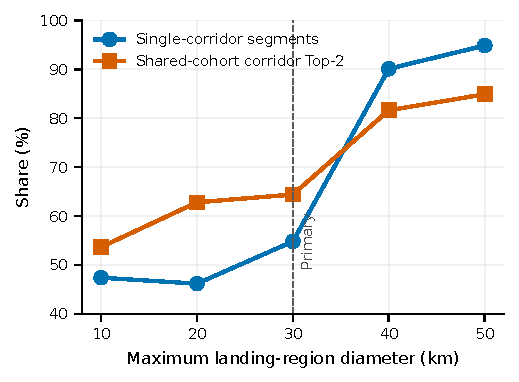
\includegraphics[width=0.84\columnwidth]{figures/fig_sensitivity_diameter.pdf}
  \caption{A-Root landing-region diameter sensitivity under a fixed 50-km
  endpoint catchment and 5-ms RTT tolerance.}
  \label{fig:diameter-sensitivity}
\end{figure}

The sweep shows a clear resolution transition. The 10--30-km settings retain
a finer coastal partition, whereas single-corridor share rises to 90.1\% and
94.8\% at 40 and 50~km and median Top-2 share reaches 81.6\% and 84.9\%.
We use 30~km because it remains on the fine side of this observed transition
while consolidating nearby facilities; 40--50~km merge substantially more
candidate support into single corridors. The A-Root check therefore supplies
an empirical basis for the reporting resolution within the tested A-Root
subset and an operational basis for the 30-km setting used throughout the
audit.

\subsection{Dependence on Geolocation and Candidate Construction}
\label{subsec:geolocation-scope}

Every projection begins with IPinfo hop geolocation and the fixed 50-km
endpoint catchment. Geographic, lifecycle, and propagation constraints then
construct the feasible candidate set. Cable lifecycle filtering aligns the
inventory with July~1, 2026; a recorded inventory refresh changed 222 of 694
cable records, including 26 planned-flag changes and 47 revised service dates.
The output retains exact landing-pair, cable, corridor, and mapping-resolution
identities, making each projected distribution traceable to its geolocation
and inventory inputs.

\subsection{Snapshot and Population Scope}
\label{subsec:measurement-scope}

All 18 measurements cover 00:00--01:00 UTC on July~1, 2026, and the
supporting datasets are aligned to the measurement date. This common
observation window supports cross-sectional comparisons among services
and geographic groups. The reported distributions describe the paths
observed during that interval.

Reported quantities are observation-weighted over participating RIPE Atlas
probes and therefore represent the probes and source ASNs present in each
country--measurement population. The eligibility thresholds of 10 probes and
3 probe ASNs remove sparse units from the paired analysis.

The service measurements retain their selected instances, while the dynamic
multi-target references deliberately sample many destinations during the same
window. The reference distributions therefore provide a broader-target
context for the service-facing populations. Anycast observations jointly
reflect deployed footprint, BGP selection, interconnection, and source-
network context.

\subsection{Implications for Diversity Measurement}
\label{subsec:resilience-implications}

A network-layer diversity summary has two distinct interpretations:
it can describe the breadth of a particular population, or rank that
population against others. The within-unit comparison measures how the
first description changes at the corridor layer; Layer Agreement measures
the correspondence between the two rankings. Stronger rank association
can coexist with substantial within-unit narrowing. Reporting both
therefore identifies what is preserved across layers without treating
ranking agreement as equality of physical breadth.

The DNS country-level summaries put the geographic rank contrast in context.
Island and archipelagic countries have a lower median corridor Top-2 share
than other coastal countries (53.3\% versus 75.4\%) and a higher median
effective corridor count (5.58 versus 3.39). Thus, the observed DNS
country-level medians show broader corridor support for the island group.
Across 38 countries with both exposure and corridor summaries, exposure
has Spearman associations of -0.29 with corridor Top-2 share and 0.30 with
effective corridor count. These statistics describe entry frequency and
conditional breadth at the country level, complementing the service-facing
unit-level Layer Agreement comparison.

A possible explanation for the geographic contrast is that maritime access
and network organization impose partly shared constraints on concentration
rankings for island and archipelagic sources. In coastal-mainland settings,
terrestrial routing, domestic backhaul, and interconnection may allow
network concentration to vary more independently of feasible submarine
corridors. This is a mechanism hypothesis; the present comparisons measure
the geographic association. Distinguishing these explanations would require
evidence linking the relevant access and routing structures to individual
country--measurement outcomes.

For diversity audits, the unit-level results provide concrete inspection
targets: 81 service-facing populations have broad network support but
concentrated corridor support, and the continuous summaries identify
additional narrowing among the 158 populations classified as broad at
both layers. The geographic comparison adds context to interpreting
network-layer rankings: they track corridor concentration more closely
in the observed island and archipelagic group than in the coastal-mainland
group. Together, these results support checking physical-corridor
concentration alongside network diversity when evaluating service paths.

Corridor concentration can be combined with cable multiplicity within a
corridor, landing-station redundancy, shared terrestrial backhaul, correlated
hazards, available rerouting capacity, and repair processes in a broader
resilience assessment. CLASP supplies the cross-layer concentration component
and preserves the exact candidate identities needed for that follow-on
analysis.

\subsection{Ethics and Reproducibility}
\label{subsec:ethics-reproducibility}

The study uses archived public RIPE Atlas measurements and infrastructure
metadata and reports aggregate country--measurement statistics. It does not
target individual users or report individual probe addresses. Candidate
assignments are feasible hypotheses and should not be interpreted as
disclosure of an operator's actual cable use.

The released measurement IDs, configuration values, mapping-resolution
states, pipeline counts, and scripts reconstruct the primary tables and
figures from versioned inputs. The paper's 80\% four-class rule is the primary
descriptive classification; the repository's tier-based auxiliary
classification uses a different rule and must remain separately named in the
artifact.
